\chapter{Overview}

The \ShellName\ is in fact a Python3 shell wrapped by \texttt{PtPython} with some useful modules, classes and methods included. This document covers those items assuming, that a reader is familiar with Python syntax.

\section{Architecture of \ShellName}

\index{\ShellName!architecture}
Look at Figure \ref{aioarchitecture}. It shows \ShellName\ wrappers from the top to the Python3 core. User calls a Bash script, which prepares and executes a command containing Python3 call, module PtPython loading, and then importing all useful libraries included in module \texttt{aio}. So to run the \ShellName\ you need to call:
\begin{alltt}
	\aio [python\_file\_name\_to\_execute]
\end{alltt}
If no argument, then the \ShellName\ appears and is ready to execute Python commands. If a script file is specified as an argument, then its content is executed after importing all modules and the shell closes. 

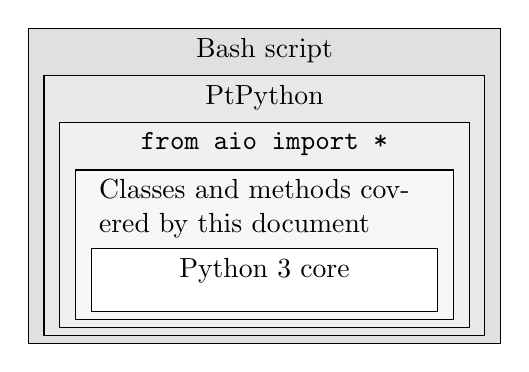
\begin{tikzpicture}
	\draw[fill=white!88!black] (-3,0) rectangle (3,-4);
	\node[anchor=north] at (0,0) {Bash script};
	\draw[fill=white!91!black] (-2.8,-0.6) rectangle (2.8,-3.9);
	\node[anchor=north] at (0,-0.6) {PtPython};
	\draw[fill=white!94!black] (-2.6,-1.2) rectangle (2.6,-3.8);
	\node[anchor=north] at (0,-1.2) {\texttt{from aio import *}};
	\draw[fill=white!97!black] (-2.4,-1.8) rectangle (2.4,-3.7);
	\node[anchor=north, text width=4.2cm] at (0,-1.8) {Classes and methods covered by this document};
	\draw[fill=white] (-2.2,-2.8) rectangle (2.2,-3.6);
	\node[anchor=north] at (0,-2.8) {Python 3 core};
\end{tikzpicture}

There is also a special mode of \ShellName, called \textbf{Testcase Mode}. It makes easy to execute a complete testcases. The testcase is a directory having a regular structure:
\dirtree{%
	.1 testcase\_name.
		.2 data \DTcomment{automatically added to the searching path}.
		.2 results \DTcomment{Created automatically by \ShellName}.
		.2 driver.py \DTcomment{Main script - your Testcase code}.
}
By running the command:
\begin{alltt}
	\daio
\end{alltt}
the \ShellName\ runs in the Testcase mode. In such case it checks if the \texttt{driver.py} file exists. If so, then it removes and recreates the \texttt{results} directory and goes there (so \texttt{results} is now the Current Directory). Now, a content of \texttt{dirver.py} is executed. In \texttt{results} directory a \texttt{transcript.txt} is created. To print something to the screen and also to the transcript file, you need to call the \texttt{print(*args)} method of class \texttt{Aio}, i.e.:
\begin{lstlisting}[language=Python]
# This text will be printed to the screen only:
print("Text on the screen only")
	
# This also appears in the transcript file:
Aio.print("Text on the screen and in the transcript")
\end{lstlisting} 

